\chapter{Plbmng Tool}
\label{chapter:plbmng}
Plbmng application called \texttt{Data miner for PlanetLab} is available at public PyPi repository\footnote{Link to PyPi repistory containing Data miner for PlanetLab tool: https://pypi.org/project/plbmng/}. The tool allows managing \texttt{PlanetLab} nodes, gathering information about them and pulling the latest data from the \texttt{PlanetLab} API service. Its core is written in Bash and additional modules are written in Python 3 \cite{suba1}. At the moment, it is depended on both Bash and Python modules and its installation consists of several steps:
\begin{itemize}
	\item Installing the application from PyPi repository or downloading the source codes from GitHub.
	\item Installing additional system packages like dialog,pssh and fping.
	\item Locating installation folder and putting symlink into \texttt{\$PATH} directory.
\end{itemize}
\section{Description of Tool's Funcionality}
First menu option is \texttt{Search nodes} for retrieving a node from internal database. This options allows user to either search by \zk{zkDNS} (\zkratkatext{zkDNS}), \zk{zkIP} (\zkratkatext{zkIP}) address or by node location. Second option is \texttt{Measure Menu} that allows user to schedule gathering of data about the nodes using \texttt{crontab}, select elements to monitor or start the data gathering right now. In the \texttt{Map Menu} option user has option to generate map showing location of the nodes and select map element. After the first start of the application user is required to fill credentials and \texttt{SSH} public key details to be able to access \texttt{PlanetLab} API and nodes using the menu option \texttt{Settings}. Menu is created using bash library \texttt{dialog} and can be seen in Figure~\ref{fig:planetlaboldmenu} and can be run directly from terminal making it available even through \texttt{ssh} client without setting up any graphical tools.

\begin{figure}[H]
	\centering
	\scalebox{0.4}{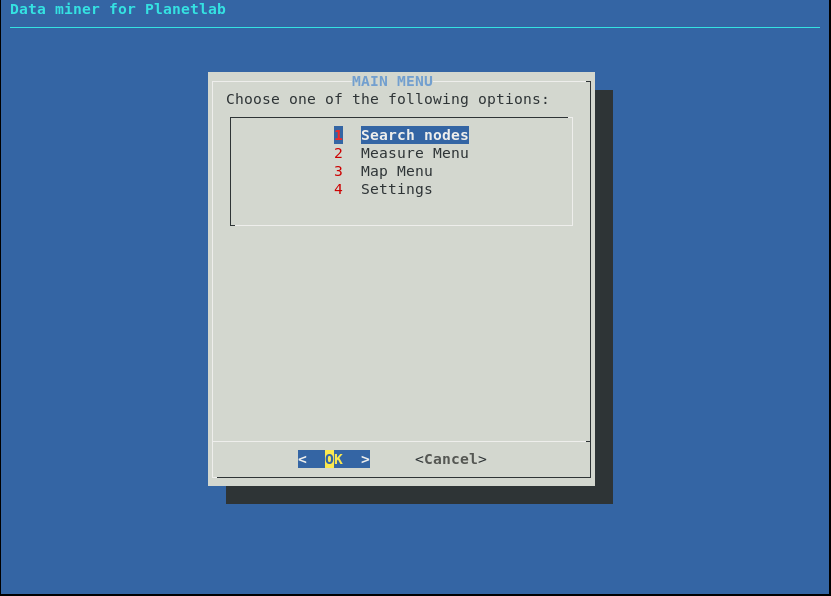
\includegraphics{obrazky/planetlabmenuold}}
	\caption{Data miner for PlanetLab menu.}
	\label{fig:planetlaboldmenu}
\end{figure}


\section{Areas of improvement}
The first problem of the existing tool is language disparity having half of the functionality in Bash and half of the functionality in Python 3. This makes it difficult to make adjustment to the tool as one needs to study a vast amount of scripts that are in several different folders. Since some of the functionality is done in Python 3, which is according to portal StackOverflow fastest-growing major programming language \cite{pythonfastestgrowing}, and because it is available at PyPi Python is an ideal candidate as a main language of the project. As a part of the semestral thesis the existing code will be re-written into Python 3.\\
Second area of improvement is installation of the tool and post-installation steps. At the moment, it is required to install additional packages and tool is not automatically put into \texttt{\$PATH} folders forcing its users to locate the installation folder and run the script from there. Because of the single programming language being \texttt{Python 3} the dependencies for system packages will be removed and their \texttt{Python 3} counter-parts will be added as dependency for the PyPi package. Pypi installer takes care of these dependencies automatically during the installation procedure. To remove post-installation steps the tool will be written as library allowing us to create an easy \texttt{Python} script in \texttt{bin} folder which is put into \texttt{\$PATH} folders by the PyPi installer during the installation.\\
Another improvements is renaming certain menu components. This change is not significant and is purely cosmetic but can make it easier for new users to get familiar with the tool. Since the tool is not data mining rather then using servers and managing them, the tool is internally renamed from \texttt{Data miner or PlanetLab} into \texttt{PlanetLab Server Manager}. Version is added next to the name for users to see immediately. Another example is renaming \texttt{Search nodes} to \texttt{Access servers} since primary function of this menu item is to access the servers while search is just supporting it.\\
The tool currently contains a lot of bugs and bad coding practices. Example of bugs is whole application crashing because of missing file when returning back from \texttt{Search nodes} menu. During the rewriting into \texttt{Python 3} there is space to improve certain controls to avoid these crashes and needs to restart the application. As for bad code practices, as an example the tool currently calls functions recursively during returning from child menu page into parent one. This means the previous function menu is stored in the \texttt{stack} waiting for the application to end before released. During rewriting of the tool these implementation details can be changed to stick with the good coding practices. 

\chapter{PlanetLab Network}
\label{chapter:planetlabnetwork}
PlanetLab is a global research network that enables the development of new network services. According to the PlanetLab project main page it was used by more than 1000 researches at top academic institutions and industrial research labs to develop a new technologies for distributed storage, network mapping, peer-to-peer systems, distributed hash tables, and query processing since it launch at 2003 \cite{planetlabmain}. The main description also states t currently consists of 1353 nodes at 717 sites \footnote{Important aspect to mention is that not all nodes are accessible. The \texttt{plbmng} tool can monitor accessibility of the nodes so its users have always overview which nodes can be actually used for their projects.}. The current committee of the project consists of members like Princeton University, Cambridge University, Intel, Google and many more \cite{planetlabmain}.\\

\section{Terminology}
During the initial planning of \texttt{PlanetLab network} the authors agreed on using common terminology for aspects of the network and defined them in the \texttt{Phase 0 document} \cite{Roscoe_PDN-02-002} as follows:
\begin{itemize}
	\item \textbf{Node:} A server machine capable of running components of PlanetLab services.
	\item \textbf{Site:} A physical geographical location where PlanetLab nodes are located.
	\item \textbf{Cluster:} The set of PlanetLab nodes located at a given site.
	\item \textbf{User:} An authorized human being wishing to deploy or run service over PlanetLab network.
	\item \textbf{Client:} A client of a service running over PlanetLab network.
	\item \textbf{Service:} An application running over PlanetLab network.
	\item \textbf{Application:} A PlanetLab service not being part of PlanetLab infrastructure. 
	\item \textbf{Capsule:} A component of a PlanetLab service that runs on a single node.
	\item \textbf{Slice:} A distributed set of resources allocated to a service in PlanetLab.
\end{itemize}
\section{PlanetLab Enabled Projects}
In this section we will shortly describe various projects that PlanetLab network enabled to create. All these projects wouldn't be possible without the resources PlanetLab brings. On PlanetLab site there is partial bibliography of research enabled by PlanetLab and it consist of over two hundred projects \cite{planetlabmain}. Having over two hundred projects enabled by PlanetLab network shows that PlanetLab had succeeded in their initial goals which was to provide a useful platform for networking and system research \cite{Roscoe_PDN-02-002}. Example of projects enabled by PlanetLab are described in the following subsections.
\subsection{Securing Web Service by Automatic Robot Detection}
This project is focusing on detection of automatic robots by implementing a special form of Touring test. Detection is done by comparing human versus robot behavior on the websites. According to the authors, 95\% of the human users can be detected within the first 57 requests \cite{Park:2006:SWS:1267359.1267382}.
\subsection{The Design and Implementation of a Next Generation Name Service for the Internet}
Project that is aiming to solve the vulnerability of the current \zk{zkDNS} (\zkratkatext{zkDNS}) and slow delivery of updates to the system. Project paper describes design and implementation of the Cooperative Domain Name System (CoDoNS), a novel name service, which provides high lookup performance through proactive caching, resilience to denial of service attacks through automatic load-balancing, and fast propagation of updates \cite{Ramasubramanian:2004:DIN:1030194.1015504}.
\subsection{Slurpie: a cooperative bulk data transfer protocol}
Big data transfers can become problematic during peaks when huge amount of clients starts downloading the data at one point. This can occur for example during a launch of a new game or a new operating system. Slurpie is is a  a peer-to-peer protocol for bulk data transfer that aims to reduce client download times of large popular files and to reduce load on the providing servers \cite{1356981}. 
\chapter{Linux and Virtualization}
\label{chapter:Linux}
\section{Linux}
In this section the operating system Linux that PlanetLab nodes are running on, and that \texttt{plbmng} tool is developed for, will be reviewed and described. Operating system is a connecting layer between hardware and software. It provides interface for work with system resources such as disk, processor or memory and at the same time it provides service layer for client software to run at. Linux is an open-source operating system originally created by Linus Torvalds who wrote it using \texttt{C language}. It was originally developed for personal computers based on the Intel x86 architecture but since its creation it has been ported to many other platforms such as mobile devices, television chips and many others. A package containing Linux operating system is called Linux distribution. The defining component of each distribution is the Linux kernel \cite{eckert2012linux+}. Original Linux kernel has been created by Linus in 1991 \cite{linuxintro} and since them many other forks of this kernel has emerged. Some of the most famous are \texttt{Red Hat Enterprise Linux},  \texttt{CentOS}, \texttt{Fedora}, \texttt{Ubuntu},  \texttt{Debian} or \texttt{SUSE Enterprise Linux}.\\
\section{Virtualization}
Virtualization 

\begin{figure}[H]
	\centering
	\scalebox{0.7}{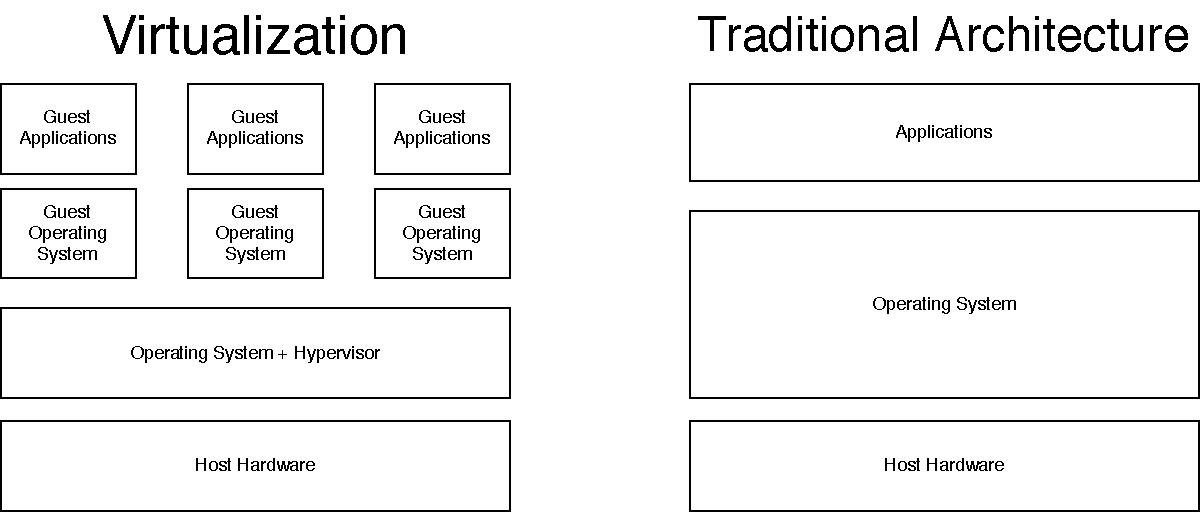
\includegraphics{obrazky/virt}}
	\caption{Virtualization vs traditional architecture schema.}
	\label{fig:virtschema}
\end{figure}


\chapter{Plbmng Tool Improvements}
\label{chapter:improve}
